\documentclass[12pt, xelatex,ja=standard,jafont=hiragino]{bxjsarticle}

\usepackage{phyexp3_robot}
\usepackage{natbib}
\usepackage{graphicx}
\usepackage{amsmath}
\usepackage{ascmac}
\usepackage{listings}
\renewcommand{\lstlistingname}{リスト}
\lstset{
  basicstyle={\ttfamily},
  identifierstyle={\small},
  commentstyle={\smallitshape},
  keywordstyle={\small\bfseries},
  ndkeywordstyle={\small},
  stringstyle={\small\ttfamily},
  frame={tb},
  breaklines=true,
  columns=[l]{fullflexible},
  numbers=left,
  xrightmargin=0em,
  xleftmargin=3em,
  numberstyle={\scriptsize},
  stepnumber=1,
  numbersep=1em,
  lineskip=-0.5ex
}
\usepackage[
 xetex,
 setpagesize=false,%
 bookmarks=true,%
 bookmarksdepth=tocdepth,%
 bookmarksnumbered=true,%
 colorlinks=true,%
 linkcolor=black,
 pdftitle={},%
 pdfsubject={},%
 pdfauthor={},%
 pdfkeywords={}%
]{hyperref}
\CJKspace

\newif\ifdraft
\draftfalse
%----
\year{2026} %実施年度
\supervisor{島田 伸敬、安藤 潤人、藤井 康之} % 担当教員



\class{D1} % クラス（D1, D2）
\date{\today}
\reportnum{1}
\assignmentnum{1, 2, 3} % 課題番号
\mailaddr{is0791pi@ed.ritsumei.ac.jp} % メールアドレス
\date{\today}
%\drafttrue % 提出時には行の先頭に% をつけて%\drafttrueとしてください

%----本文はここから---

\begin{document}
\maketitle
\section{ロボットプログラミングテーマの内容}
\ifdraft
（この文章は58行目の\verb|\drafttrue|をコメントアウトすると消える）

ここにロボットプログラミングのテーマ内容について、自分なりにまとめて200字程度で説明を記載すること。どういう実験内容か、何を学ぶか、など。 以下の各実験課題の結果についても、データや画像、プログラムコードを貼り付けるだけでなく、それぞれの説明をレポートとして記載すること。
それらがどの程度充実しているかが評価につながる。

キャプチャ画像の解像度が高すぎるとファイルのサイズが20MBを超えてしまいmanaba+Rにアップロードできなくなる。解像度を下げることと（低すぎて見づらくならないように）PNG画像よりもJPG画像を用いるほうがよい。

\fi
% 以下に本文を書く
本実験ではROS(RObot Operating System)を使った移動ロボットを用いて，その仕組みとSLAM(Simultaneous Localization And Mapping)による環境地図の作成やこれを用いたロボットの誘導，さらにはPythonを連携させたロボットのマニピュレーションについて学ぶ．またこれらの実験をLinuxコマンドラインを用いて行うことで，CLIによるソフトウェア利用に対する理解を深め，その技能を習得する．

\section{課題1: ロボットの操作とROSの基礎}

\subsection{課題1-1}
\begin{screen}
リモコン操作でロボットの動きをよく観察しなさい。リモコンからの入力はどういう信号に変換されて送られていると思うか（位置、速度、加度など）。各キーにバインドされた制御信号を予想して下に記載しなさい。
\end{screen}
\paragraph{回答欄：予想}
% 以下に本文を書く
リモコンの各キーに割り当てられた動作についての予想を，各キー毎に述べていく．
\begin{itemize}
    \item 「U,D,L,R」キー
\end{itemize}
それぞれ「前進」「後退」「左旋回」「右旋回」の動作が実行される．これらのキーは最大6回を上限に，押す毎にその動作は速くなったことから，リモコンから送られる信号はモータの角速度を増減させる命令を持っていると考えた．
\begin{itemize}
    \item 「1」キー
\end{itemize}
アームに取り付けられた手先モジュールの動きを制御するキーである．1回押すたびに手が開くか閉じるかの動作を行う．この開閉の動作は１つのモータによって実装されていたため，このキーを押したときリモコンからの入力はこのモータに一定量の回転をさせる命令を実行していると考えた．例えば手が開くときに$+θ(rad)$の回転をおこなったならば，閉まるときには$-θ(rad)$の回転をおこなっている．
\begin{itemize}
    \item 「2,4」キー
\end{itemize}
それぞれアームの「左旋回」「右旋回」の動作が実行されている．これらのキーは長い時間押し続けた方が回転量が多かったことから，ロボットの動作を実装するループ関数が存在し，この1回のループの中で1回のみこれらのキーの入力状態が判定されアームの回転が実現していると考えた．
\begin{itemize}
    \item 「3」キー
\end{itemize}
アームを上下に動かすためのキーである．前述の「1」キーと同様に1回押すたびにアームが下がるか上がるかの動作を行う．

%ここにアームの構造をかいて，それに関する考察を書く%

\begin{itemize}
    \item 「5」キー
\end{itemize}
このキーを押すとロボットは移動に関する動作を全て停止する．移動に関わる全てのモータの角速度を$0$にしているものと考えられた．

\subsection{課題1-2}
\begin{screen}
\href{https://wiki.ros.org/ja/ROS/Tutorials/UnderstandingTopics}{チュートリアルサイトの「ROSトピックの理解」}のページを開いて，教員の説明を聞きながら順を追ってROS環境操作の各手順を実行し、内容を理解しなさい。その後、rostopic pubコマンドを使ってturtlesimのタートルを一定の並進速度・回転速度で動かす命令（ただしチュートリアルサイトの数字とは違う速度の指示値を与えよ）を実行して、そのときのrostopicコマンドの文字列と実行後のタートル表示ウインドウをキャプチャして下に貼りなさい。
\end{screen}

\paragraph{回答欄：実行したコマンド列}
% 以下に本文を書く
\ifdraft %以下は例
実行したコマンド列をリスト\ref{lst:command}に示す。
\begin{lstlisting}[caption=実行したコマンド列,label=lst:command]
command...
command...
\end{lstlisting}
\fi

\paragraph{回答欄：コマンド実行後に表示されたタートルの軌跡}
% 以下に本文を書く
\ifdraft %以下は例
コマンド実行後に表示されたタートルの軌跡を図\ref{fig:turtle}に示す。\\
これは例なので、自分で試した画像を添付すること。
% 以下に画像を貼る
\begin{figure}[htb]
    \centering
    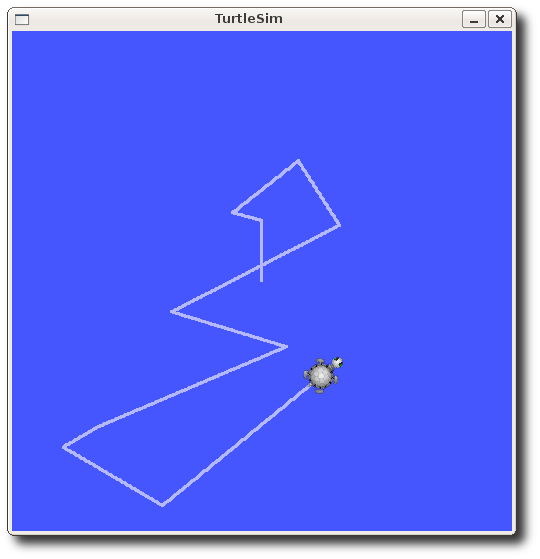
\includegraphics[width=0.7\linewidth]{images/turtle_key.png}
    \caption{タートルの軌跡}
    \label{fig:turtle}
\end{figure}
\fi

\paragraph{回答欄：実行コマンド列とタートルの軌跡についての説明（詳しく）}
% 以下に本文を書く

\subsection{課題1-3}
\begin{itembox}[l]{(1)}
\href{https://wiki.ros.org/ja/ROS/Tutorials/WritingPublisherSubscriber%28python%29}{「シンプルな配信者(Publisher)と購読者(Subscriber)を書く」チュートリアル}に記載されている指示に従いtalker.pyとlistener.pyをダウンロードするか直接ファイルにコピーペーストして保存しなさい。
\end{itembox}

\paragraph{回答欄：talker.pyのコードを貼り付ける}
talker.pyのコードをリスト\ref{lst:talker.py}に示す。
\begin{lstlisting}[caption=talker.py,label=lst:talker.py]
    #!/usr/bin/env python
    # license removed for brevity
    import rospy
    from std_msgs.msg import String

    def talker():
        pub = rospy.Publisher('chatter', String, queue_size=10)
        rospy.init_node('talker', anonymous=True)
        r = rospy.Rate(10) # 10hz
        while not rospy.is_shutdown():
            str = "hello world %s"%rospy.get_time()
            rospy.loginfo(str)
            pub.publish(str)
            r.sleep()

    if __name__ == '__main__':
        try:
            talker()
        except rospy.ROSInterruptException: pass
\end{lstlisting}

\paragraph{回答欄：listener.pyのコードを貼り付ける}
listener.pyのコードをリスト\ref{lst:listener.py}に示す。
\begin{lstlisting}[caption=listener.py,label=lst:listener.py]
    #!/usr/bin/env python
    import rospy
    from std_msgs.msg import String

    def callback(data):
        rospy.loginfo(rospy.get_caller_id()+"I heard %s",data.data)
        
    def listener():

        # in ROS, nodes are unique named. If two nodes with the same
        # node are launched, the previous one is kicked off. The 
        # anonymous=True flag means that rospy will choose a unique
        # name for our 'listener' node so that multiple listeners can
        # run simultaenously.
        rospy.init_node('listener', anonymous=True)

        rospy.Subscriber("chatter", String, callback)

        # spin() simply keeps python from exiting until this node is stopped
        rospy.spin()
            
    if __name__ == '__main__':
        listener()
\end{lstlisting}

\begin{itembox}[l]{(2)}
保存した2つのプログラムを指示に従って動かして、どういう動作をするか確かめなさい(ターミナルを開いてrosrunコマンドを使う)。どのような出力が得られたかを下に示し、そこから確認できる動作の内容を説明しなさい。
\end{itembox}


\paragraph{回答欄：出力結果とその説明}
% talker.py とlistener.py.を実行したときの出力結果を貼り付ける（画像でも可）
% コードや出力結果等に関する説明を記述
% 以下に本文を書く
\ifdraft %以下は例
talker.py とlistener.py.を実行したときの出力結果をリスト\ref{lst:output_talkerpy}に示す。X行目では... Y行目では
\begin{lstlisting}[caption=出力結果,label=lst:output_talkerpy]
output...
output...
output...
\end{lstlisting}
\fi

talker.pyとlistener.pyを実行した時の出力結果を，それぞれ図\ref{fig:talker},\ref{fig:listener}で示す．

\begin{figure}
    \centering
    \includegraphics[width=0.75\linewidth]{images/}
    \label{fig:talker}
\end{figure}
\begin{figure}
    \centering
    \includegraphics[width=0.75\linewidth]{images/}
    \label{fig:listener}
\end{figure}

\subsection{課題1-4}
\begin{itembox}[l]{(1)}
授業中の解説を参考に、キーボードで入力したテキスト文字を送受信するROSノードをpython(rospy)を使って実装しなさい。python2ではキーボード入力の取得に\verb|raw_input()|が使える。
\end{itembox}


\begin{itembox}[l]{(2)}
そのコード（クライアント：talker2.py）を示せ(もしlistener.pyを修正していたなら、listener2.pyとしてそのコードも示すこと）。さらにtalker2.pyをどのように改変したのか、その内容を詳しく説明すること。
\end{itembox}

\paragraph{回答欄：talker2.py}
% 以下に本文を書く
\ifdraft %以下は例
改変したクライアントtalker2.pyをリスト\ref{lst:talker2}に示す。
\begin{lstlisting}[caption=実行したコマンド列,label=lst:talker2]
#!/usr/bin/env python
# license removed for brevity
import rospy
from std_msgs.msg import String

def talker():
    pub = rospy.Publisher('chatter', String, queue_size=10)
    rospy.init_node('talker', anonymous=True)
    r = rospy.Rate(10) # 10hz
    while not rospy.is_shutdown():
        str = "hello world %s"%rospy.get_time()
        rospy.loginfo(str)
        pub.publish(str)
        r.sleep()

if __name__ == '__main__':
    try:
        talker()
    except rospy.ROSInterruptException: pass
\end{lstlisting}
\fi

\paragraph{回答欄：talker2.pyの改変内容の説明}
%以下に本文をかく

\paragraph{回答欄：listener2.py}
% 以下に本文を書く
listener.pyには変更を加えていない。
\ifdraft
listener.pyを変更した場合はここにコードを示すこと
\fi

\begin{itembox}[l]{(3)}
テキストの送受信に使用されるトピック名と、送受信メッセージの定義（rosmsgコマンドを使用せよ）を添付せよ。
\end{itembox}
\paragraph{回答欄：トピック名と，送受信メッセージの定義}
% 以下に本文を書く
\ifdraft
トピック名と送受信メッセージの定義を貼り付ける。
メッセージの定義についての説明を自分の言葉で書く。
\fi

\begin{itembox}[l]{(4)}
実行した時の画面表示をキャプチャ、貼り付けた上でその説明をせよ。
\end{itembox}

\paragraph{回答欄：実行した時の画面表示}
% 実行した時の画面表示を貼り付け、それについて詳しく説明する
% 以下に本文を書く
\ifdraft %以下は例
作成したプログラムの実行画面を図\ref{fig:rosmsg}に示す（この画面はだいぶ違うが）。このプログラムではテキストをXXXというトピックにおいてYYYしており...
% 以下に画像を貼る
\begin{figure}[htb]
    \centering
    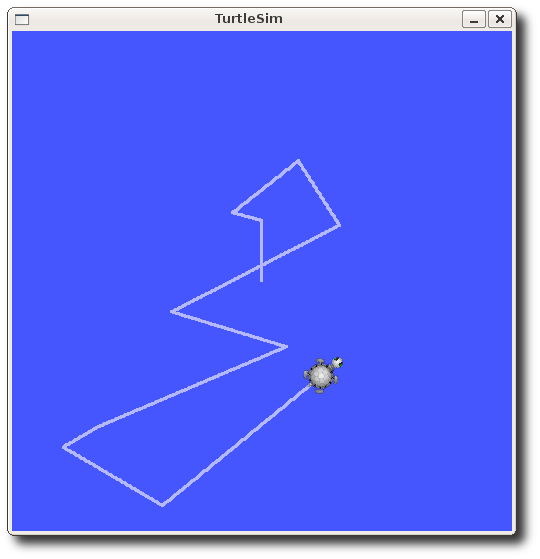
\includegraphics[width=0.7\linewidth]{images/turtle_key.png}
    \caption{テキストの送受信を行うプログラムの実行画面}
    \label{fig:rosmsg}
\end{figure}
\fi

\begin{itembox}[l]{(5)}
\verb|rostopic echo|コマンドを実行して、流れているROSメッセージを端末に表示し、それをキャプチャして添付しなさい（画像でもテキストでもよい）。
\end{itembox}

\paragraph{回答欄：実行した時の画面表示}
\ifdraft
リスト\ref{lst:rostopic_echo}にrostopic echoコマンドの実行結果を示す。X行目に...

\begin{lstlisting}[caption=rostopic echoの実行結果,label=lst:rostopic_echo]
msg: 
  message
\end{lstlisting}
\fi

\begin{itembox}[l]{(6)}
\verb|rqt_graph|コマンドを実行して、ノード・トピックの関係図を表示し、画像として添付したうえで説明しなさい。
\end{itembox}

\paragraph{回答欄：ノード・トピックの関係図とその説明}
\ifdraft
\verb|rqt_graph|コマンド実行後に表示されるノード・トピックの関係図\ref{fig:rqtgraph}に示す。
このコマンドは現在実行されているノードとトピックを示しており、ノードは...

\begin{figure}[htb]
    \centering
    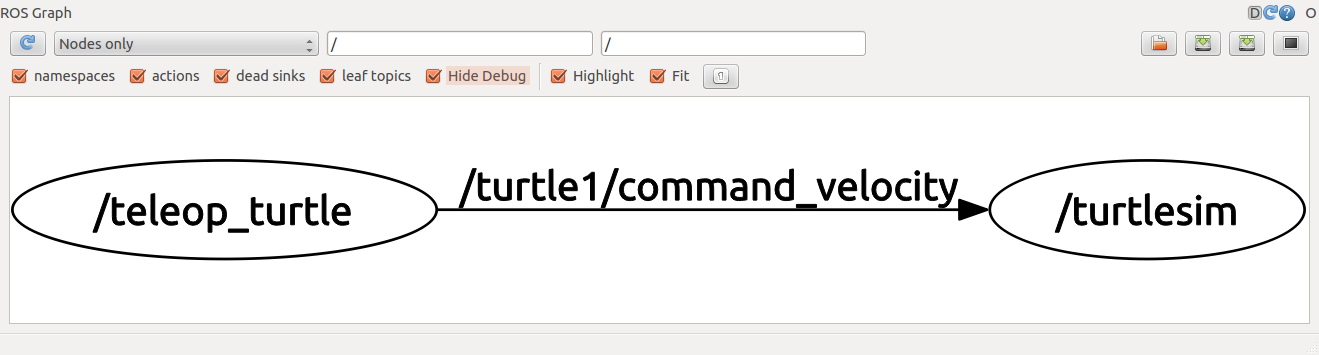
\includegraphics[width=0.7\linewidth]{images/rqt_graph_turtle_key.png}
    \caption{ノード・トピックの関係図}
    \label{fig:rqtgraph}
\end{figure}
\fi

\begin{itembox}[l]{(7)}
talker2.pyを複数起動すると，2ノード以上からのテキストをlistener.pyは表示することができる．実際に試してみて，なぜそれが可能なのか考察し説明せよ．
\end{itembox}

\paragraph{回答欄：考察・説明}
\ifdraft
考察・説明を詳しく記述する
\verb|rqt_graph|のグラフで2ノード以上のtalker2.pyが動いている様子を示すとわかりやすい
\fi

\subsection{課題1-5}
\begin{screen}
talker2.pyとlistener.py(もしくはlistener2.pyなど）のpythonコードを参考に，双方向でテキストを送受信できるように改造したPython
プログラムを実装し、回答欄に貼り付けた上で、そのコードを説明せよ。   
\end{screen}


\paragraph{回答欄：Pythonコードとその説明}
\ifdraft
リスト\ref{lst:python_bidirectinal}に双方向でテキストを送受信可能なサービスとクライアントのコードを示す。6行目に定義したtalkerメソッドでは... listenerメソッドでは、メッセージを受信して表示する...

\begin{lstlisting}[caption=双方向でテキストを送受信可能なサービスとクライアント,label=lst:python_bidirectinal]
#!/usr/bin/env python
# license removed for brevity
import rospy
from std_msgs.msg import String

def talker():
    pub = rospy.Publisher('chatter', String, queue_size=10)
    rospy.init_node('talker', anonymous=True)
    r = rospy.Rate(10) # 10hz
    while not rospy.is_shutdown():
        str = "hello world %s"%rospy.get_time()
        rospy.loginfo(str)
        pub.publish(str)
        r.sleep()

if __name__ == '__main__':
    try:
        talker()
    except rospy.ROSInterruptException: pass
\end{lstlisting}
\fi

\begin{screen}
発展として教員のPCで起動しているroscoreに接続し、文字列を送ってみた場合は、教員からの応答や自動応答の様子、\verb|rqt_graph|による接続の様子などをキャプチャして動作の様子を説明せよ
\end{screen}
\paragraph{回答欄：発展課題の説明}
\ifdraft
発展として教員のPCで起動したノードに対してトピック通信を行うことを試みた。方法は...
\fi

\newpage
\section{課題2: GazeboシミュレーションによるTurtlebot3の操作}
\subsection{課題2-1}
\begin{screen}
Gazeboシミュレータ(gazebo.launch)とRViz(rviz.launch)、teleop(teleop.launch)を起動してTurtlebotを適当に移動させ、その時のGazeboの画面（視点を自由に移動せよ）、RVizの画面をキャプチャして添付せよ。
\end{screen}
\paragraph{回答欄：Gazeboの画面とRVizの画面}
\ifdraft
Gazeboの画面とRVizの画面を図\ref{fig:gazebo}に示す。
この画面は...

\begin{figure}[htb]
    \centering
    
\includegraphics[width=0.7\linewidth]{images/blank.png}
    \caption{Gazeboの画面とRVizの画面}
    \label{fig:gazebo}
\end{figure}
\fi

\subsection{課題2-2}
\begin{screen}
\verb|rosnode list|コマンドを実行してどのようなノードが起動しているか確認し、結果を添付せよ。また、各ノードがどういうものかわかる範囲で調べて説明せよ。
\end{screen}
\paragraph{回答欄：ノードとその説明}
\ifdraft
ノードを貼り付ける。画像でも可。
また、各ノードがどういうものかわかる範囲で調べて説明する。
\fi

\subsection{課題2-3}
\begin{screen}
\verb|rostopic list|コマンドを実行して、どのようなトピックが作られているか確認し、結果を添付せよ。また、各トピックのうち2、3のトピックを選び、そのトピックの役割をわかる範囲で調べて説明せよ。
\end{screen}
\paragraph{回答欄：トピックとその説明}
\ifdraft
トピックのリストを貼り付ける。画像でも可。
各トピックのうち２〜３のトピックを選び、そのトピックの役割をわかる範囲で調べて説明する。
\fi

\subsection{課題2-4}
\begin{screen}
\verb|rostopic echo|コマンドを実行して、いくつかのトピックメッセージが流れている様子を観察せよ。観察したトピック名とその内容（大量に流れるので10行程度で良い）を添付せよ。また、選んだトピックに流れるメッセージの内容をみて、どういう情報が何の目的で流されているのかわかる範囲で調べて説明せよ。
\end{screen}
\paragraph{回答欄：トピック名とその内容、および、その内容の説明}
\ifdraft
トピック名とその内容を貼り付ける(画像でも可)。
選んだトピックに流れるメッセージの内容をみて、どういう情報が何の目的で流されているのかわかる範囲で調べて説明する。
\fi

\subsection{課題2-5}
\begin{screen}
teleop.launchや各種コマンドを駆使して，Turtlebot3への行動命令が流れているトピックを特定せよ。そのトピック名と、メッセージの型名、メッセージの定義(rosmsg showコマンドを用いよ）を添付せよ。また、どのようにしてそのトピックを特定したのか、その過程と特定理由について説明せよ。
\end{screen}

\paragraph{回答欄：トピック名と，メッセージの型名，メッセージの定義、および、トピックの特定過程と理由}
\ifdraft
トピック名と，メッセージの型名，メッセージの定義を貼り付ける(画像でも可)。
また、トピックを特定するに至った過程と理由について詳しく説明する。
\fi

\subsection{課題2-6}
\begin{screen}
\verb|rqt_graph|コマンドを実行して、ノード・トピックの関係図を表示し、画像として添付せよ。
\end{screen}

\paragraph{回答欄：ノード・トピックの関係図}
\ifdraft
ノード・トピックの関係図を図\ref{fig:rqt2}に示す。
この図では...

\begin{figure}[htb]
    \centering
    
\includegraphics[width=0.7\linewidth]{images/blank.png}
    \caption{ノード・トピックの関係図}
    \label{fig:rqt2}
\end{figure}
\fi

\newpage
\section{課題3: 実機Turtlebotへの接続と移動操作}
\subsection{課題3-1}
\begin{screen}
Turtlebot実機に接続してノードを起動し（machine.launch)、教室のブロックフィールドに実機を置いてteleopで移動させよ。適当なところで停止させ、その様子を撮影した写真とその時のRVizの画面を添付せよ。
\end{screen}
\paragraph{回答欄：撮影した写真とその時のRVizの画面}
\ifdraft
撮影した写真を図\ref{fig:photo_turtlebot}に、またその時のRVizの画面を図\ref{fig:rviz_turtlebot}に示す。

\begin{figure}[htb]
    \centering
    
\includegraphics[width=0.7\linewidth]{images/blank.png}
    \caption{Turtlebotの実機写真}
    \label{fig:photo_turtlebot}
\end{figure}
\begin{figure}[htb]
    \centering
    
\includegraphics[width=0.7\linewidth]{images/blank.png}
    \caption{Turtlebot起動中のRVizの画面}
    \label{fig:rviz_turtlebot}
\end{figure}
\fi

\subsection{課題3-2}
\begin{screen}
距離センサの反応する範囲にものを設置して動かし、距離センサの反応がRVizの画面上で変化していることを比較して確認せよ。この時の実環境の様子とRVizの画面をキャプチャして添付し、様子を文章で説明せよ（2つの異なる状況でセンサの反応が異なっていることがわかる画像を\textbf{2種類}添付すること）．
\end{screen}
\paragraph{回答欄：実環境の様子とRVizの画面、および、その説明}
\ifdraft
図\ref{fig:photo_turtlebot_proximity}は距離センサにXを近づけている様子を撮影したものである。図\ref{fig:rviz_turtlebot_proximity}はその時のRVizの画面である...

\begin{figure}[h]
\centering
\begin{minipage}[b]{0.49\columnwidth}
    \centering
    
\includegraphics[width=1\linewidth]{images/blank.png}
    \caption{距離センサの反応（通常時）：実機の様子}
    \label{fig:photo_turtlebot_normal}
\end{minipage}
\begin{minipage}[b]{0.49\columnwidth}
    \centering
    
\includegraphics[width=1\linewidth]{images/blank.png}
    \caption{距離センサの反応（通常時）：RVizの画面}
    \label{fig:rviz_turtlebot_normal}
\end{minipage}
\end{figure}

\begin{figure}[h]
\centering
\begin{minipage}[b]{0.49\columnwidth}
    \centering
    
\includegraphics[width=1\linewidth]{images/blank.png}
    \caption{距離センサの反応（近づけたとき）：実機写真}
    \label{fig:photo_turtlebot_proximity}
\end{minipage}
\begin{minipage}[b]{0.49\columnwidth}
    \centering
    
\includegraphics[width=1\linewidth]{images/blank.png}
    \caption{距離センサの反応（近づけたとき）：RVizの画面}
    \label{fig:rviz_turtlebot_proximity}
\end{minipage}
\end{figure}
\fi



%\bibliographystyle{plain}
%\bibliography{references}
\end{document}

